\chapter{Área de Estudo}
\label{cap:area_estudo}

A área de estudo compreende os estados de São Paulo (SP) e Rio Grande do Norte (RN), localizados, respectivamente, nas regiões Sudeste e Nordeste do Brasil (Figura~\ref{fig:mapa_clima_brasil}). A seleção dessas unidades federativas fundamenta-se na representatividade de regimes climáticos contrastantes dentro do território brasileiro, evidenciada por diferenças fisiográficas, hidrológicas e climáticas significativas. São Paulo caracteriza-se pelo predomínio de climas subtropicais úmidos (Cfa, Cwa, Cwb), enquanto o Rio Grande do Norte apresenta predominância de clima semiárido quente (BSh) no interior e clima tropical úmido (As) na faixa litorânea (Figuras~\ref{fig:mapa_clima_sp} e~\ref{fig:mapa_clima_rn}), sendo estas classificações explicadas a partir da Tabela \ref{tab:koppen_classes}. Essa diversidade abrange distintos biomas e padrões de uso e cobertura da terra, possibilitando análises comparativas de variabilidade e mudanças climáticas em contextos ambientais diferenciados. A caracterização climática regional é apresentada com base na classificação de Köppen-Geiger \citep{alvares2013, Kottek2006}, enquanto os aspectos relacionados aos biomas e ao uso da terra seguem a classificação oficial dos biomas brasileiros e mapeamentos recentes de uso e cobertura da terra \citep{ibge_biomas2004,ibge_biomas_pagina,mapbiomas_collection8_platform}.

\section{Caracterização Climática}

\begin{table}[h!]
\centering
\caption{Descrição das classes climáticas segundo a classificação de Köppen-Geiger. 
A primeira letra indica o grupo climático principal, a segunda o regime de precipitação 
e a terceira (quando presente) o regime térmico.}
\label{tab:koppen_classes}

\renewcommand{\arraystretch}{1.2} % aumenta espaçamento vertical

\begin{tabular}{cl}
\hline
\textbf{Sigla} & \textbf{Descrição} \\
\hline

\multicolumn{2}{l}{\textbf{Climas Tropicais (A)}} \\
Af  & Tropical úmido \\
Am  & Tropical de monção \\
Aw  & Tropical com estação seca \\
As  & Tropical com verão seco \\[4pt]

\multicolumn{2}{l}{\textbf{Climas Secos (B)}} \\
BSh & Semiárido quente \\[4pt]

\multicolumn{2}{l}{\textbf{Climas Subtropicais (C)}} \\
Cfa & Subtropical úmido \\
Cfb & Subtropical oceânico \\
Cwa & Subtropical com inverno seco \\
Cwb & Subtropical de altitude \\
Csa & Mediterrâneo quente \\

\hline
\end{tabular}
\end{table}


O Brasil apresenta grande diversidade climática em função de sua extensão territorial, variação latitudinal e características fisiográficas (Figura~\ref{fig:mapa_clima_brasil}). Segundo a classificação de Köppen-Geiger \citep{alvares2013, Kottek2006}, o território brasileiro abrange desde climas tropicais úmidos (Af, Am, Aw) predominantes na região Norte e em parte da faixa litorânea, passando por climas semiáridos (BSh) característicos do interior nordestino, até climas subtropicais (Cfa, Cfb, Cwa, Cwb) que ocorrem nas regiões Sul e Sudeste. As principais classes climáticas e suas características estão descritas na Tabela~\ref{tab:koppen_classes}. Essa classificação leva em consideração o abordado no material disponibilizado pelo \cite{forestgis2015} que disponibiliza a classificação Köppen-Geiger em formato shapefile, podendo ser utilizado via malhas no software QGIS.

\begin{figure}[h!]
\centering
\fbox{\includegraphics[width=0.85\textwidth]{fig/mapa_bio.png}}
\caption[Classificação climática de Köppen-Geiger no Brasil.]
{Distribuição espacial dos tipos climáticos segundo a classificação de Köppen-Geiger no território brasileiro. Observa-se ampla diversidade climática, com predomínio de climas tropicais úmidos (Af, Am, Aw) na Amazônia e costa atlântica norte, climas semiáridos (BSh) no sertão nordestino, e climas subtropicais (Cfa, Cfb, Cwa, Cwb) nas regiões Sul e Sudeste. Os estados de São Paulo e Rio Grande do Norte, encontram-se em destaque com contornos em vermelho (detalhamento nas Figuras~\ref{fig:mapa_clima_sp} e~\ref{fig:mapa_clima_rn}). Fonte: \cite{alvares2013, Kottek2006}, adaptado via QGIS.}
\label{fig:mapa_clima_brasil}
\end{figure}

\begin{figure}[h!]
\centering
\fbox{\includegraphics[width=0.85\textwidth]{fig/mapa_sp_bio.png}}
\caption[Classificação climática de Köppen-Geiger no estado de São Paulo.]
{Distribuição espacial dos tipos climáticos segundo a classificação de Köppen-Geiger no estado de São Paulo. O estado apresenta predominância de climas subtropicais, com destaque para o tipo Cfa (subtropical úmido sem estação seca) no centro-sul e litoral, Cwa (subtropical com inverno seco) no interior e planalto ocidental, e Cwb (subtropical de altitude com inverno seco) em regiões serranas e de maior elevação. Pequenas áreas com clima tropical (Am, Aw) ocorrem no extremo norte, enquanto o tipo Cfb (subtropical oceânico) aparece em porções da Serra da Mantiqueira e litoral sul. Fonte: \cite{alvares2013, Kottek2006}, adaptado via QGIS.}
\label{fig:mapa_clima_sp}
\end{figure}

\begin{figure}[h!]
\centering
\fbox{\includegraphics[width=0.85\textwidth]{fig/mapa_rn_bio.png}}
\caption[Classificação climática de Köppen-Geiger no estado do Rio Grande do Norte.]
{Distribuição espacial dos tipos climáticos segundo a classificação de Köppen-Geiger no estado do Rio Grande do Norte. O estado caracteriza-se pelo predomínio do clima semiárido quente (BSh) em praticamente todo o interior, ocupando a maior extensão territorial. Na faixa litorânea, observa-se a transição para climas tropicais, com presença do tipo As (tropical com verão seco) no litoral oriental e norte, e pequenas áreas de clima Aw (tropical com inverno seco) no extremo sul. Essa configuração reflete o gradiente de precipitação do litoral para o interior. Fonte: \cite{alvares2013, Kottek2006}, adaptado via QGIS.}
\label{fig:mapa_clima_rn}
\end{figure}

No estado de São Paulo (Figura~\ref{fig:mapa_clima_sp}), observa-se a predominância de climas subtropicais úmidos, com variações espaciais associadas à altitude, à continentalidade e à proximidade com o oceano Atlântico. A porção centro-sul do estado e a faixa litorânea são caracterizadas pelo clima Cfa (subtropical úmido sem estação seca), com precipitação bem distribuída ao longo do ano e verões quentes. Na faixa litorânea, a presença da Serra do Mar contribui para o aumento da precipitação orográfica, mantendo elevados totais pluviométricos mesmo nos meses mais secos. No interior e no planalto ocidental, predomina o clima Cwa (subtropical com inverno seco), caracterizado por uma estação seca bem definida entre os meses de abril e setembro, com concentração das chuvas no período de verão. Nas regiões de maior altitude, como a Serra da Mantiqueira e porções elevadas da Serra do Mar, ocorre o clima Cwb (subtropical de altitude com inverno seco), que se diferencia do Cwa por apresentar verões mais amenos devido à elevação topográfica.

No Rio Grande do Norte (Figura~\ref{fig:mapa_clima_rn}), predominam condições climáticas semiáridas em praticamente todo o interior do estado, caracterizadas pelo clima BSh (semiárido quente). Este domínio climático apresenta elevada irregularidade espacial e temporal da precipitação, com totais anuais geralmente inferiores a 800 mm e forte variabilidade interanual. A estação chuvosa concentra-se nos meses de fevereiro a maio, período de maior atuação da Zona de Convergência Intertropical (ZCIT), principal sistema indutor de precipitação na região. Na faixa litorânea oriental e norte do estado, observa-se a transição para climas tropicais, com predomínio do tipo As (tropical com verão seco). Este padrão, menos comum entre os climas tropicais, caracteriza-se por uma estação seca que ocorre nos meses de verão (setembro a fevereiro), com a estação chuvosa concentrada no outono-inverno. Pequenas áreas no litoral sul apresentam o clima Aw (tropical com inverno seco), padrão mais típico dos climas tropicais brasileiros. Essa configuração climática reflete um gradiente de precipitação do litoral para o interior, associado à atuação diferenciada de sistemas atmosféricos.
\newpage
\section{Localização Geográfica e Caracterização Fisiográfica}

O estado de São Paulo situa-se entre aproximadamente 19°S e 25°S de latitude e 44°W e 53°W de longitude, abrangendo uma área de cerca de 248.200 km$^2$. O relevo paulista é caracterizado pela predominância de planaltos e depressões, com destaque para o Planalto Atlântico, a Depressão Periférica Paulista e as faixas serranas da Serra do Mar e da Serra da Mantiqueira. Essas feições topográficas exercem influência direta sobre os padrões de circulação atmosférica regional, a distribuição da precipitação e os gradientes térmicos, especialmente em função dos efeitos orográficos e da proximidade com o Oceano Atlântico \citep{ibge_biomas_pagina}.

O clima predominante no estado é o subtropical úmido, com estação chuvosa bem definida durante a primavera e o verão austral, associada principalmente à atuação da Zona de Convergência do Atlântico Sul (ZCAS) e à passagem de sistemas frontais. A estação seca ocorre preferencialmente durante o inverno, quando a atuação de sistemas de alta pressão reduz a ocorrência de precipitação. A precipitação média anual apresenta elevada variabilidade espacial, com totais superiores a 1.600 mm em áreas serranas e litorâneas e valores inferiores a 1.200 mm em regiões do interior \citep{coelho2016}.

O estado do Rio Grande do Norte localiza-se entre aproximadamente 4°S e 7°S de latitude e 34°W e 38°W de longitude, com área aproximada de 52.800 km$^2$. O relevo é predominantemente plano a suavemente ondulado, com presença de planaltos residuais e depressões sertanejas, o que resulta em menor influência orográfica sobre a precipitação quando comparado ao Sudeste brasileiro \citep{ibge_biomas_pagina}.

O clima do Rio Grande do Norte varia do tropical úmido na faixa litorânea ao semiárido no interior do estado. A precipitação apresenta forte irregularidade espacial e temporal, com totais médios anuais superiores a 1.200 mm no litoral oriental e valores inferiores a 600 mm em extensas áreas do sertão. A dinâmica climática regional é fortemente influenciada pela Zona de Convergência Intertropical (ZCIT), além de teleconexões oceânicas associadas às anomalias de temperatura da superfície do mar no Atlântico tropical \citep{marengo2017}.

\section{Biomas e Uso e Cobertura da Terra}

A caracterização dos biomas e das classes de uso e cobertura da terra neste estudo baseia-se nos dados do projeto MapBiomas \citep{mapbiomas_atbd_c8,souza2020_mapbiomas}, que fornece séries históricas anuais de uso e cobertura da terra para todo o território brasileiro a partir de imagens de sensoriamento remoto e algoritmos de classificação automatizada.

As classes de uso e cobertura da terra consideradas neste estudo seguem a legenda oficial do projeto MapBiomas (Coleção 9), contemplando formações naturais, áreas antrópicas e superfícies não vegetadas. A descrição dessas classes, bem como seus respectivos códigos, é apresentada na Tabela~\ref{tab:mapbiomas_classes}, permitindo a correta interpretação dos mapas temáticos apresentados a seguir.

\begin{table}[H]
\centering
\caption[Classes de uso e cobertura da terra do MapBiomas.]
{Descrição das classes de uso e cobertura da terra adotadas neste estudo, conforme a legenda oficial do projeto MapBiomas (Coleção 9, segundo catálogo de classes disponível em: \url{https://brasil.mapbiomas.org/wp-content/uploads/sites/4/2024/08/Legenda-Colecao-9-LEGEND-CODE.pdf}). A coluna de cores corresponde à simbologia utilizada nos mapas temáticos apresentados.}
\label{tab:mapbiomas_classes}
\begin{minipage}{0.48\textwidth}
\centering
\begin{tabular}{c c l}
\hline
\textbf{Código} & \textbf{Cor} & \textbf{Classe} \\
\hline
3  & \cellcolor[RGB]{31, 141, 73}  & Formação Florestal \\
4  & \cellcolor[RGB]{125, 201, 117}  & Formação Savânica \\
5  & \cellcolor[RGB]{4, 56, 29}  & Mangue \\
6 & \cellcolor[RGB]{0, 119, 133}   & Floresta Alagável \\
12  & \cellcolor[RGB]{214, 188, 116} & Formação Campestre \\
15 & \cellcolor[RGB]{237, 222, 140} & Pastagem \\
20 & \cellcolor[RGB]{219, 112, 147}  & Cana \\
21 & \cellcolor[RGB]{255, 239, 195}   & Mosaico de Usos \\
23 & \cellcolor[RGB]{255, 160, 122} & Praia, Duna e Areal \\
24 & \cellcolor[RGB]{212, 39, 30}    & Área Urbanizada \\
25 & \cellcolor[RGB]{219, 77, 79}    & Outras Áreas não Vegetadas \\
29 & \cellcolor[RGB]{255, 170, 95}  & Afloramento Rochoso \\
32 & \cellcolor[RGB]{252, 129, 20}  & Apicum \\
\hline
\end{tabular}
\end{minipage}
\hfill
\begin{minipage}{0.48\textwidth}
\centering
\begin{tabular}{c c l}
\hline
\textbf{Código} & \textbf{Cor} & \textbf{Classe} \\
\hline
30 & \cellcolor[RGB]{156, 0, 39}  & Mineração \\
31 & \cellcolor[RGB]{9, 16, 119} & Aquicultura \\
33 & \cellcolor[RGB]{37, 50, 228}   & Rio, Lago e Oceano \\
39 & \cellcolor[RGB]{245, 179, 200} & Soja \\
40 & \cellcolor[RGB]{199, 21, 133}   & Arroz \\
41 & \cellcolor[RGB]{245, 76, 169}   & Outras Lavouras Temporárias \\
46 & \cellcolor[RGB]{214, 143, 226}  & Café \\
47 & \cellcolor[RGB]{153, 50, 204} & Citrus \\
48 & \cellcolor[RGB]{245, 76, 169} & Outras Lavouras Perenes \\
49 & \cellcolor[RGB]{122, 89, 0} & Silvicultura \\
50 & \cellcolor[RGB]{2, 214, 89} & Restinga Arbórea \\
62 & \cellcolor[RGB]{255, 105, 180} & Algodão (beta) \\
75 & \cellcolor[RGB]{255, 255, 255}   & Não observado \\
\hline
\end{tabular}
\end{minipage}
\end{table}

No estado de São Paulo, o bioma predominante era a Mata Atlântica, originalmente caracterizada por florestas densas e elevada biodiversidade \citep{ribeiro2009_atlanticforest}. Entretanto, a cobertura florestal remanescente encontra-se altamente fragmentada em decorrência de séculos de ocupação antrópica, restando atualmente uma fração reduzida da vegetação original \citep{sos_inpe_atlas}. O uso da terra no estado é dominado por atividades agropecuárias, especialmente agricultura mecanizada e pastagens, além de extensas áreas urbanizadas concentradas na Região Metropolitana de São Paulo e em polos industriais do interior.

\begin{figure}[H]
\centering
\fbox{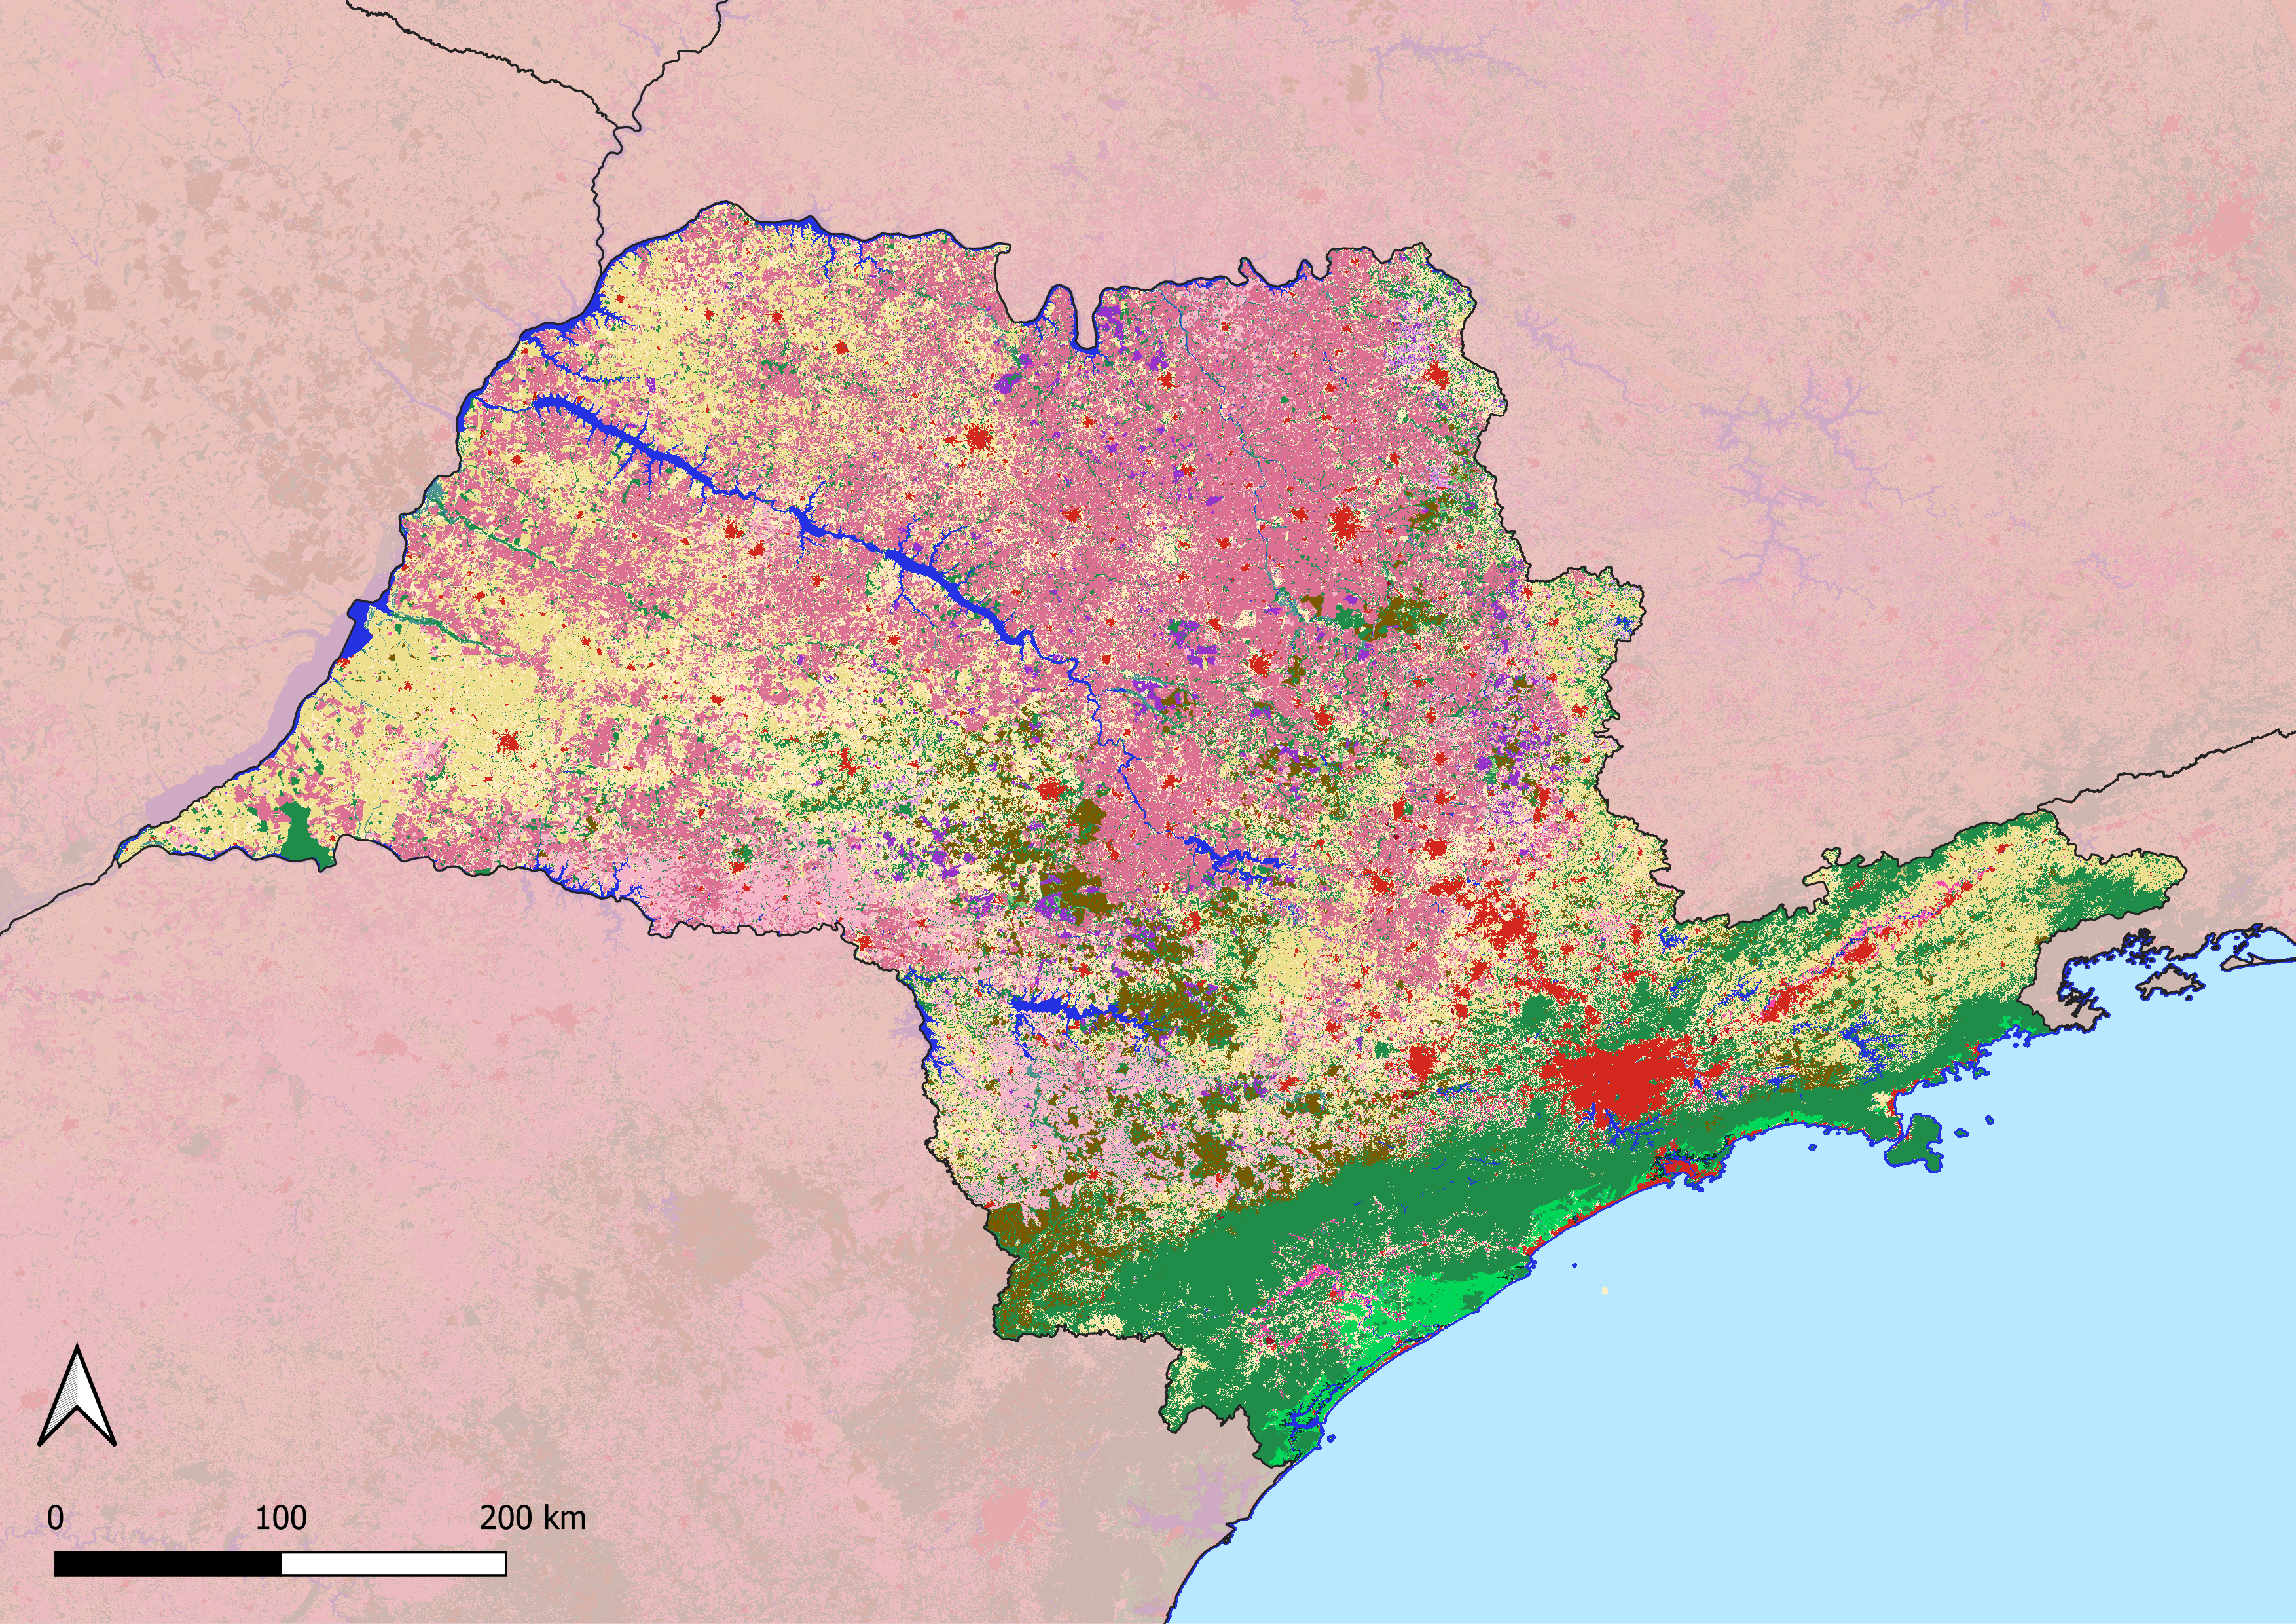
\includegraphics[width=0.9\textwidth]{fig/mapa_sp.png}}
\caption[Uso e cobertura da terra no estado de São Paulo.]
{Mapa de uso e cobertura da terra do estado de São Paulo, elaborado a partir da Coleção 9 do projeto MapBiomas (ano-base 2024). Fonte: Autor com auxílio do complemento MapBiomas Collection Official via QGIS.}
\label{fig:mapa_uso_sp}
\end{figure}

Com base na Figura~\ref{fig:mapa_uso_sp}, observa-se o predomínio de usos antrópicos no interior do estado, com destaque para as classes Pastagem, Cana e Mosaico de Usos (Tabela~\ref{tab:mapbiomas_classes}), associadas principalmente à atividade agropecuária. Os remanescentes de vegetação nativa concentram-se majoritariamente na faixa litorânea e em áreas serranas.

No estado do Rio Grande do Norte, o bioma Caatinga predomina na maior parte do território estadual, caracterizando-se por vegetação adaptada a condições semiáridas, elevada sazonalidade fenológica e forte dependência do regime de chuvas \citep{leal2003_caatinga}. Na faixa litorânea oriental, ocorre o bioma Mata Atlântica, associado a ambientes de maior umidade e à presença de ecossistemas costeiros, como manguezais e restingas \citep{ibge_biomas2004}. Assim como observado em São Paulo, o estado apresenta alterações significativas na cobertura vegetal natural decorrentes da expansão agropecuária, da urbanização costeira e da exploração de recursos naturais.

\begin{figure}[H]
\centering
\fbox{\includegraphics[width=0.9\textwidth]{fig/mapa_rn.png}}
\caption[Uso e cobertura da terra no estado do Rio Grande do Norte.]
{Mapa de uso e cobertura da terra do estado do Rio Grande do Norte, elaborado a partir da Coleção 9 do projeto MapBiomas (ano-base 2024). Fonte: Autor com auxílio do complemento MapBiomas Collection Official via QGIS.}
\label{fig:mapa_uso_rn}
\end{figure}

De acordo com a Figura~\ref{fig:mapa_uso_rn}, observa-se o predomínio de formações naturais associadas ao bioma Caatinga no interior do estado, intercaladas por áreas de uso agropecuário extensivo, principalmente Pastagem e Mosaico de Usos (Tabela~\ref{tab:mapbiomas_classes}). Na faixa litorânea, destacam-se áreas urbanizadas, remanescentes de Mata Atlântica e ecossistemas costeiros, refletindo condições climáticas mais úmidas e maior pressão antrópica.